\documentclass[10pt, twocolumn]{article}

% --- Packages ---
\usepackage[utf8]{inputenc}
\usepackage[english]{babel}
\usepackage[margin=0.75in]{geometry} % Optimized margins for 2-page limit
\usepackage{graphicx}
\usepackage{booktabs} % For beautiful tables
\usepackage{amsmath}
\usepackage{hyperref}
\usepackage{titlesec}
\usepackage{abstract}

% --- Clickable Links Config ---
\hypersetup{
    colorlinks=true,
    linkcolor=blue,
    filecolor=magenta,      
    urlcolor=blue,
}

% --- Compact Headings ---
\titlespacing{\section}{0pt}{*2}{*1}
\titlespacing{\subsection}{0pt}{*1}{*1}

% --- Title Information ---
\title{\vspace{-1.5cm}\textbf{Idemia Datachallenge (IADATA704): \\ Face Occlusion Prediction}}
\author{
    \textbf{Group Name:} Team GPU \\
    \textbf{Group Number:} 21 \\
    \textbf{Team Members:} Oscar DE LA CRUZ, Rémi HAMON
}

\date{    
    %\fbox{
        \parbox{\textwidth}{
            \centering
            \textbf{Project repository:}
            \url{https://github.com/odelacruz-fierro/data-challenge-idemia.git}
        }
    %}
    \vspace{-0.5cm}
}


\begin{document}

\maketitle

% ===================================================
% --- Introduction
% ===================================================
\section{Introduction}
In the context of the Data Challenge proposed by Idemia, the objective is to predict the percentage of facial occlusion
in images (224x224 pixels). The major challenge lies in handling the training data imbalance (a low proportion of the training database
contain highly occluded faces) and the gender fairness requirement imposed by the evaluation metric.

In this report, we present our solution based on multi-task learning and data augmentaion, designed to extract robust features
while minimizing the demographic bias penalty.

% ===================================================
% --- Exploratory Data Analysis
% ===================================================
\section{Exploratory Data Analysis}
\label{sec:eda}

The exploratory data analysis (EDA) performed on the train database revealed that only a low proportion of the faces show a high occlusion.
This is verified by Fig.\ref{fig:train_occlusion_distribution}, where we can observe a right-skewed distribution: the samples are more concentrated
on the lower values than in the extreme high values, whici drag the tail towards the right side.

A closer look to different occlusion levels (see Table \ref{tab:occlusion_intervals}) allows us to notice that the majority of images concentrate
in the occlusion interval $[0.0,0.5]$ with a minority of them in $(0.5,1.0]$. In order to understand what thes intervals looked-like, four
occlusion levels were proposed: \textbf{low} $\in [0.0, 0.2]$, \textbf{medium-low} $\in (0.2, 0.4]$, \textbf{medium-high} $\in (0.4, 0.5]$ and
\textbf{high} $\in (0.5, 1.0]$. Sample images for these intervals are provided in figure \ref{fig:occlusion_mosaic}.
%

\begin{itemize}
    \item \textbf{low} occluded images trend to provide a global visibility of the face forehead, eyes, nose, chicks and chin.
    \item \textbf{medium-low} and \textbf{medium-high} occluded images par of the faces are covered either with the hair, a hat,
    hand, fingers and even physical objects.
    \item Finally in \textbf{high} occluded images faces seem to be mostly visible, however a blurry / noised effect was noticed. 
\end{itemize}


\begin{figure}[ht]
    \centering
    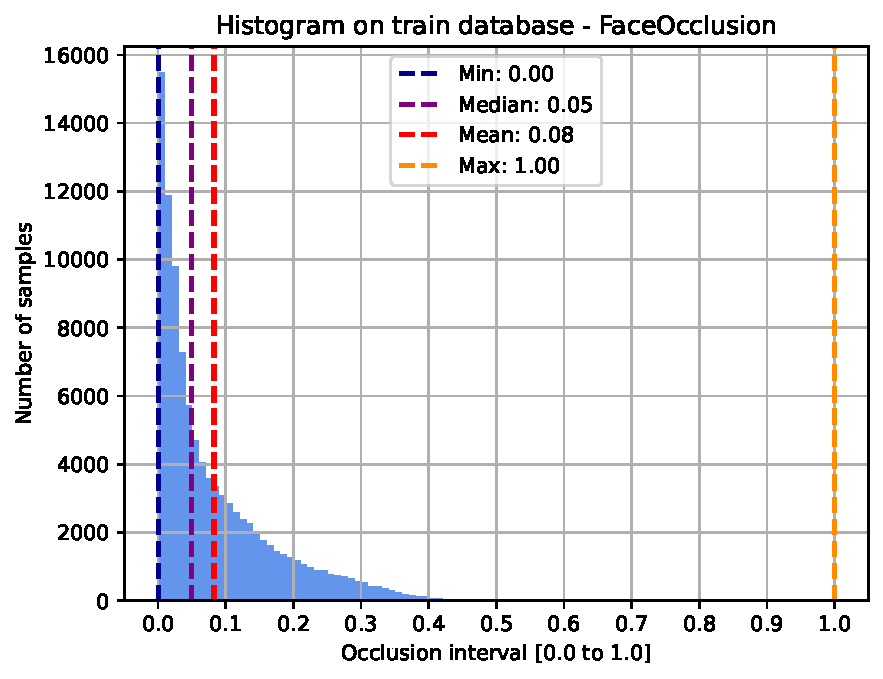
\includegraphics[width=0.9\columnwidth]{figures/occlusion_distribution.pdf}
    \caption{Distribution of occlusion across the training database.}
    \label{fig:train_occlusion_distribution}  
\end{figure}


\begin{table}[ht]
\centering
\caption{Distribution of images across occlusion intervals in the training database}
\label{tab:occlusion_intervals}
\begin{tabular}{lrc}
\toprule
\textbf{Occlusion interval} & \textbf{Image Count} & \textbf{(\%)} \\
\midrule
$[0.00, 0.10]$ & 68,929 & 68.93\% \\
$(0.10, 0.20]$ & 19,558 & 19.56\% \\
$(0.20, 0.30]$ &  8,372 &  8.37\% \\
$(0.30, 0.40]$ &  2,865 &  2.86\% \\
$(0.40, 0.50]$ &    240 &  0.24\% \\
$(0.50, 0.60]$ &     26 &  0.03\% \\
$(0.60, 0.70]$ &      5 &  0.01\% \\
$(0.70, 0.80]$ &      2 &  0.00\% \\
$(0.80, 0.90]$ &      0 &  0.00\% \\
$(0.90, 1.00]$ &      3 &  0.00\% \\
\midrule
\textbf{Total} & \textbf{100,000} & \textbf{100.00\%} \\
\bottomrule
\end{tabular}
\end{table}

\begin{figure}[ht]
    \centering
    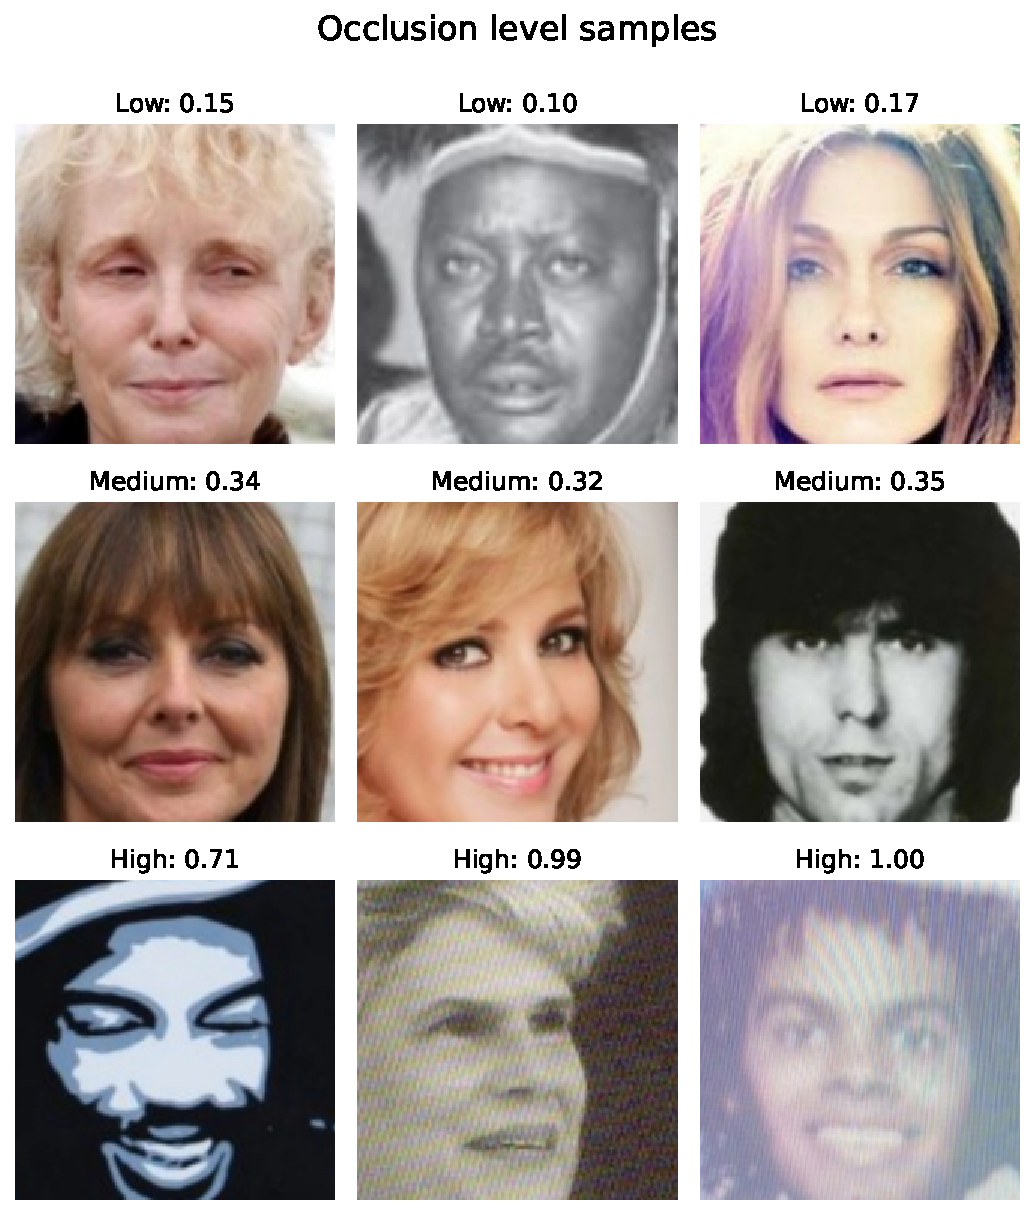
\includegraphics[width=0.9\columnwidth]{figures/occlusion_mosaic.pdf}
    \caption{Random samples for four occlusion intervals.}
    \label{fig:occlusion_mosaic}
\end{figure}


From a gender perspective, it was found that the train database contains 67.6 \% of men and 32.4 \% of women (see Fig.\ref{fig:gender_distribution}).

\begin{figure}[ht]
    \centering
    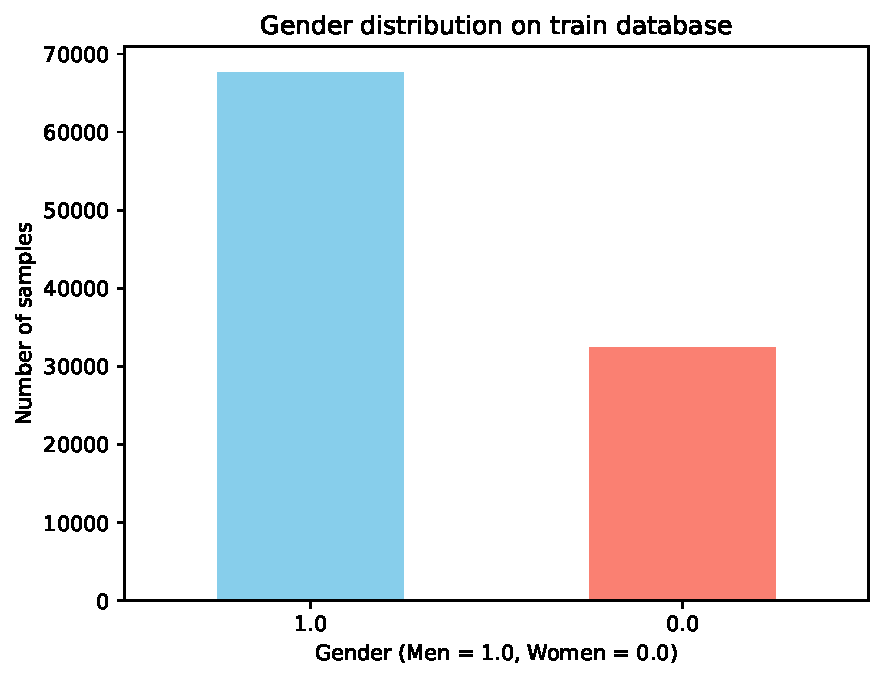
\includegraphics[width=0.9\columnwidth]{figures/gender_distribution.pdf}
    \caption{Distribution of gender across the training dataset: Men = 67.6 \% and Women = 32.4 \%.}
    \label{fig:gender_distribution}
\end{figure}






% ===================================================
% --- Section
% ===================================================
\section{Methodology \& Architecture}
\textit{TO DO ...}

% ---------------------------------------------------
% --- Subsection
% ---------------------------------------------------
\subsection{Milti-Task Learning (MLT)}
\textit{TO DO ...}
%Although the primary task is a simple regression (occlusion score), we opted for a two-head architecture. As demonstrated in the literature, the addition of an auxiliary task acts as a regularizer. The first head predicts the occlusion (via a Sigmoid activation), while the second predicts gender. This structure forces the shared feature extractor to focus on deep semantic facial features.


% ---------------------------------------------------
% --- Subsection
% ---------------------------------------------------
\subsection{Backbone architectures}
\textit{TO DO ...}

%Nous avons utilisé \texttt{MobileNetV3-Small} pré-entraîné sur ImageNet comme tronc commun. Ce choix s'explique par sa légèreté, permettant des itérations rapides.
%\\ \textbf{THIS PART WILL EVOLVE !!!}

% ===================================================
% --- Training strategy
% ===================================================
\section{Training strategy}

\textit{TO DO ...}

% ---------------------------------------------------
% --- Custom Loss
% ---------------------------------------------------
\subsection{Custom loss}
\textit{TO DO ...}
%Pour aligner notre modèle avec la métrique d'Idemia, nous avons implémenté une \textit{Weighted Mean Squared Error} (MSE). Les échantillons avec une forte occlusion vraie ($GT_i$) reçoivent un poids supérieur selon la formule $w_i = \frac{1}{30} + GT_i$.


% ---------------------------------------------------
% --- Data augmentation
% ---------------------------------------------------
\subsection{Data augmentation}
\label{sec:data-augmentation}

Often real-world data sets are predominately composed of ``normal'' examples with only a small percentage
of ``abnormal'' or ``interesting'' examples. The goal of this section is to increase the diversity of the train database in order
to match close enough the distribution of the test database (see Fig.\ref{fig:test_occlusion_distribution}).


\begin{figure}[ht]
    \centering
    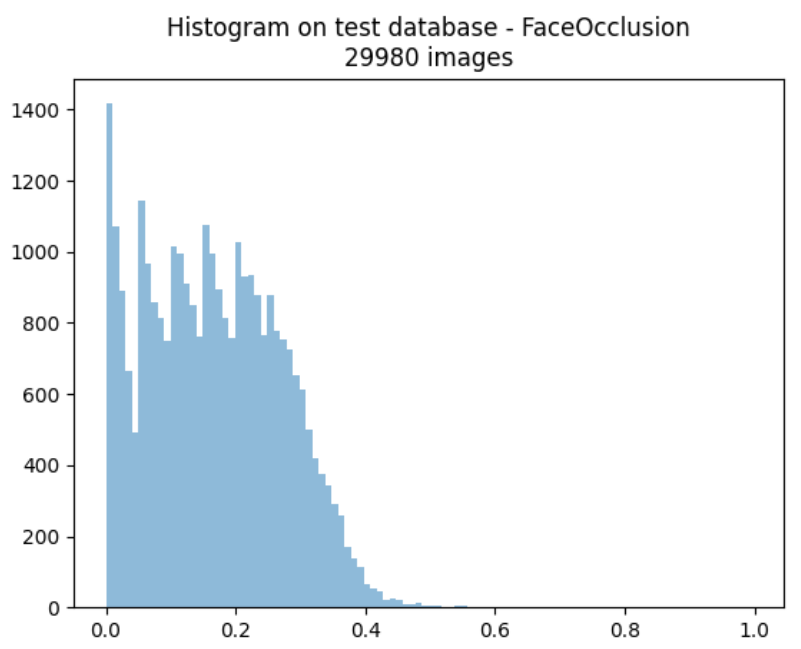
\includegraphics[width=0.9\columnwidth]{figures/hist_test_database.png}
    \caption{Distribution of occlusion across the test database.}
    \label{fig:test_occlusion_distribution}
\end{figure}

Visual analysis of the sampled intervals (see section \ref{sec:eda}) revealed a distinct dichotomy in the training data: true structural occlusions
(e.g., hands, helmets, instruments, and hair) dominate the $[0.20, 0.50]$ range, whereas values above $0.50$ consist primarily
of quality degradations such as severe sensor pixelation and artistic filter artifacts. Given that the target test distribution
concentrates heavily below $0.50$, we prioritize \texttt{RandomErasing} as our primary spatial regularizer to simulate realistic
object boundaries, treating \texttt{GaussianBlur} as a secondary augmentation to handle baseline quality invariance.

%"Although predicting face occlusion is inherently a regression task, the extreme right-skew of the target
%distribution presents a continuous class imbalance problem. To address this, we employed techniques
%traditionally reserved for classification—specifically, target discretization to calculate inverse frequency
%weights for our data sampler..." 

Reference test \cite{xu_comprehensive_2023}

Reference test \cite{chen_gridmask_2020}

Reference test \cite{chawla_smote_2002}

% ===================================================
% --- Results
% ===================================================
\section{Results}
\textit{TO DO ...}

%Notre modèle a été évalué sur le sous-ensemble "interim" du Leaderboard. Le tableau \ref{tab:results} résume nos performances.

%\begin{table}[h]
%    \centering
%    \begin{tabular}{lcc}
%        \toprule
%        \textbf{Modèle} & \textbf{MSE Validation} & \textbf{Score Leaderboard} \\
%        \midrule
%        Baseline (MSE) & 0.045 & 0.01250 \\
%        Ours (Custom Loss) & 0.021 & \textbf{0.00115} \\
%        \bottomrule
%    \end{tabular}
%    \caption{Comparaison des approches implémentées.}
%    \label{tab:results}
%\end{table}

% ===================================================
% --- Limitations and tradeoffs
% ===================================================
\section{Limitations and tradeoffs}

%Bien que performante, notre solution présente plusieurs limites :
%\begin{itemize}
%    \item \textbf{Complexité de l'hyper-paramétrage :} L'approche Multi-Tâches nécessite de régler manuellement le poids relatif ($\lambda$) entre la perte d'occlusion et la perte de genre. Un mauvais équilibrage détériore les deux métriques.
%    \item \textbf{Sensibilité au Biais Initial :} Si le \textit{batch size} est trop petit, la pénalité de \textit{fairness} fluctue énormément d'une époque à l'autre.
%    \item \textbf{Puissance de Calcul :} L'architecture actuelle est légère (MobileNet), mais des tentatives d'utilisation de modèles plus profonds (ResNet50, Swin Transformers) ont été limitées par nos ressources de calcul locales avant le passage sur le cluster.
%\end{itemize}

% ===================================================
% --- Limitations and tradeoffs
% ===================================================
\section{Conclusion}
\textit{TO DO ...}

%Notre approche démontre qu'une fonction de perte ciblée couplée à une régularisation par Multi-Task Learning permet de répondre efficacement aux contraintes spécifiques d'Idemia. Des travaux futurs pourraient inclure un \textit{Oversampling} dynamique pour annuler totalement la pénalité de genre.

% --- References ---
% \bibliographystyle{plain}
% \bibliography{references} % Uncomment if you use a .bib file
% --- References ---
\bibliographystyle{unsrt} 
\bibliography{references}


\end{document}